%
% Charset: utf8
% Content type: Plain LATEX
% Content: This chapter describes how the bootloader 'Barebox' functions and
%          how to modify things to get Barebox to work properly.
%
% Copyright Jürgen Beisert <jbe@pengutronix.de>, 2011
%
% This work is licensed under the Creative Commons Attribution 3.0 Unported License.
% To view a copy of this license, visit:
%           http://creativecommons.org/licenses/by/3.0/
% or send a letter to:
% Creative Commons, 444 Castro Street, Suite 900, Mountain View, California, 94041, USA.
%
% Refer the file CREDITS for all people working on this document.
%
% This file content will be part of the "OSELAS.BSP-Pengutronix-Mini2440-Quickstart.pdf"
%
% Note: This document uses some externaly defined LATEX commands. If you try to
% run LATEX only on this file it will fail due to the absense of these commands
% All these new commands are starting with 'ptxdist'.
%

\section{Notes About the Bootloader Barebox}	\label{sec:bareboxnotes}

Everything mentioned here (variable names and file names) in the run-time
environment that Barebox uses, is for convenience only. The developers of Barebox
decided to provide a generic run-time environment that satisfies the most
common requirements. All descriptions below will refer to this generic
run-time environment and it's behaviour.

There are no restrictions in how to adapt this environment for one's own
needs. How Barebox enters it's shell is compiled-in. Changing the
\texttt{/env/bin/init}, allows one to modify Barebox's behaviour.

%
% Idea: Describe the way from the /env/bin/init script to the booting kernel
% - where are the parameters from
% - how to change the boot source
%

\subsection{Run-Time Environment}			\label{sec:bbenv}

The Barebox binary handles only target initialization and provides device
drivers and various commands to do things after the initialization. It is up to
the user to use these features to make her/his target work. This works on a
shell code base. For example Barebox, tries to run the \texttt{/env/bin/init}
script right after the initialization is finished. This file is expected
as a part of the environment.

From the technical point of view, the Barebox environment is a simple
archive which contains files and directories. At startup, this archive will
be extracted to the \texttt{env/} directory and can be used afterwards on a
regular file base. Note: the \texttt{/} directory in Barebox is a RAM
filesystem.

As Barebox tries to run the \texttt{/env/bin/init} script after the
initialization, an environment is always required. The archive that each
environment is based on, can be a compiled-in component or can be loaded at
run-time from a persistent media.

The compiled-in environment archive is a read only archive defined at
compile-time of Barebox. The environment archive from the persistent
media is (most of the time) a read/write archive. It can be changed at any
time and saved back to make the change persistent.

Barebox always tries to load the environment archive from the registered
persistent media first. If this fails, Barebox defaults to the compiled-in
environment archive.

% Idea: Describe the components of the default environment provided by the
% Barebox source tree. What variables/scripts are used and their meaning

\subsection{How does the Partitioning Work in Barebox}	\label{sec:bbpartitioning}

Partitioning is a way to handle large media in smaller logical units. This
simplifies updates of different components and leaves others untouched. For
example, one can update the kernel to fix a bug in a driver but keep the
root filesystem unchanged. Also, redundant boot can be realized with more than
one partition per component.

%
% Idea: Add a description what "redundant boot" means
%

Barebox uses partitioning of the available persistent media (for example, NOR
or NAND flash, but also harddisks or SD cards) to handle and store the
required parts to make a target work.

Some of the available persistent media can store it's partition information on
the media itself. For example hard disks, compact flash cards or SD cards can
provide their own partition table.

In this case, Barebox can read back this table from the media and handle
these partition's sizes and locations in a correct manner.

But, there are still some media that do not provide this kind of partition table.
The well known plain flash devices (of type NOR or NAND) are such candidates.
These devices need slightly different handling. The most common method the
kernel uses is the \textit{Command line partition table parsing} for the MTD
(Memory Technology Devices) devices. A user gives a kernel parameter with the
list of names and sizes that describes the partition layout of the
corressponding flash memory.

%
% How to describe this? If Barebox do not use the plain flash, there is no need
% to partitioning it. This is the case if a target comes with NOR _and_ NAND
% memory and starts from the NOR. If Barebox does not touch the NAND flash memory,
% there is no need to partition it. On the other hand, for NOR flash we need some
% kind of partitioning. In this case, because we are starting from this memory,
% we must protect the bootloader from accidental erasure.
%

Barebox uses the same syntax to describe the partition and kernel layout. So,
a user only has to define the layout once. It will be shared between Barebox
and the Linux kernel. If one doesn't use consistent layout, one could destroy
the data in one partition by changes in another parition.

This partition layout string is defined to:

\begin{ptxshell}[escapechar=|]{^}
<size>(<name>)[,<size>(<name>)[,<size>(<name>)]...]
\end{ptxshell}

\texttt{<size>} is a number followed by its unit. The unit can be \texttt{k} for
\textit{kilobyte}, \texttt{M} for \textit{megabyte} and \texttt{G} for
\textit{gigabyte}. For \texttt{<size>} also the special letter \texttt{-}
can be given. This means, fill the remaining space up to the end of the media. The
\texttt{<name>} can be anything one likes, but must not contain any spaces!

Here is the most common partition layout configuration:

In Barebox's run-time environment it looks like:

\texttt{256k(barebox),64k(bareboxenv),2048k(kernel),-(root)}

\begin{itemize}
 \item bootloader itself (\textit{barebox}): this binary brings up the target
  after power on or reset
 \item persistent environment (\textit{bareboxenv}): used by Barebox to bring up
  the whole system in the way that the user has configured it
 \item operating system (\textit{kernel}): the kernel image, Barebox will load
  and run it
 \item root filesystem (\textit{root}): used by the kernel as the root
  filesystem
\end{itemize}

The size and location of some of these partitions can be modified at run-time
via the variable \texttt{nand\_parts} in the \texttt{env/config} file. Here the
user can increase the kernel partition, or add more partitions to the
\textit{free part} of the list.

However, two of the listed partitions are special: the location and size of
the bootloader (\textit{barebox}) partition and of the run-time environment
(\textit{bareboxenv}) partition.
%
% "[...] \textbf{AND} the location of the kernel."
%
% No, this partition is not fixed in its location. It just starts after the
% 'bareboxenv' partition. OK!
%

These must be known soon after reset. So, we have a chicken/egg problem: to
read the persistent environment, Barebox must know where the persistent environment
is located. To do so, Barebox initially creates the \textit{barebox} and
\textit{bareboxenv} partitions and after loading the persistent environment
Barebox then adds the \textbf{remaining} partitions based on the
\texttt{nand\_parts} variable.

This handling implies the internally registered partitions for Barebox and the
persistent environment must be the same in size and location as the partitions
described in the \texttt{nand\_parts} variable.

This then means, if one would like to change the size of the \textit{barebox}
or the \textit{bareboxenv} partitions, she/he must change the platform source
code \textbf{and} the \texttt{nand\_parts} variable.

Here an example for a partition setup in the run-time environment:

\begin{ptxshell}[escapechar=|]{^}
nand_parts="256k(barebox),64k(bareboxenv),2048k(kernel),-(root)"
\end{ptxshell}

It corresponds to the following NAND partition layout:

\centerline{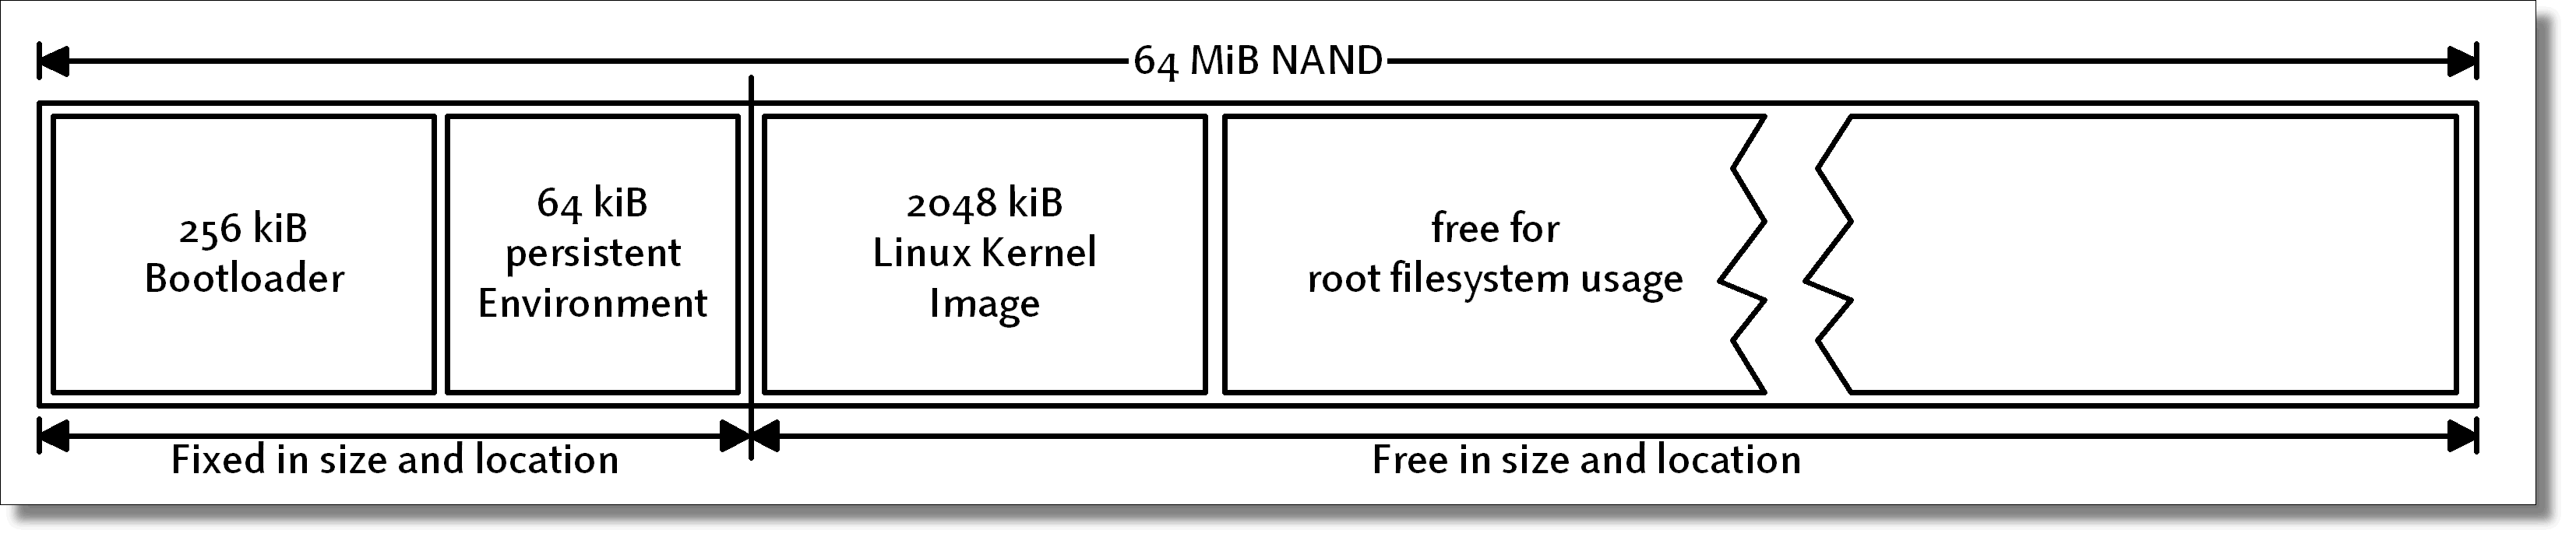
\includegraphics{OSELAS.BSP-Pengutronix-Mini2440/documentation/plain_sources/partitioning.png}}

This setup defines

\begin{itemize}
 \item 256 kiB for the bootloader (\textit{barebox}) at the beginning of the
  persistent media.
 \item 64 kiB for the persistent environment (\textit{bareboxenv}) following
  the bootloader partition
 \item 2 MiB for the kernel (\textit{kernel})
 \item the remaining space on the persistent media for the root filesystem
  (\textit{root})
\end{itemize}

For the Mini2440 the platform source code is located in:

\texttt{platform-mini2440/build-target/barebox-<version>/arch/arm/boards/mini2440/mini2440.c}

and looks like this:

\begin{ptxshell}[escapechar=|]{^}
[...]
      /* ----------- add some vital partitions -------- */
   devfs_del_partition("self_raw");
   devfs_add_partition("nand0", 0x00000, 0x40000, PARTITION_FIXED, "self_raw");
   dev_add_bb_dev("self_raw", "self0");

   devfs_del_partition("env_raw");
   devfs_add_partition("nand0", 0x40000, 0x10000, PARTITION_FIXED, "env_raw");
   dev_add_bb_dev("env_raw", "env0");
[...]
\end{ptxshell}

Please ensure after changing any of the "Fixed in size and location" partitions
that Barebox is re-compiled and re-flashed to keep the compiled-in environment
in sync with the platform source code.

Also consider: for the partitions that are free in size and location, you can
change these settings at run-time and store it to the persistent environment.
But, if this persistent environment gets lost Barebox will default to the
compiled-in environment. If this compiled-in environment has different
partition sizes and locations, error messages will occur. This is because
reading from partitions with wrong settings in size and location will fail.

So, the best procedure is to change the compiled-in environment to ensure the
partition layout is always consistent, even if the modified persistent
environment gets lost.
